% Template GRASS newsletter - Article Language: Latex LA This
% project aims to define a settlement's use of, and impact on, their
% surrounding landscape.

% Head

\title{LA} \subtitle{Identifying Landuse Catchments for 
ancient settlements.}
\author{by Jason Jorgenson and Tim Sutton}
\maketitle
\section{Introduction} \label{sec:Introduction}
  This paper describes a software application we are developing that automates
  the process of computing landuse requirements and identifying the land likely 
  to have been engaged by the people living in ancient settlements.
  The useage of the LA application is illustrated in this text using an
  archaeological site at Shuna (Figure \ref{fig:shunaGoogleEarth}) in the
  Jordan Valley.  The Jordan Valley is found in the Southern Levant, which is a name
  commonly used to refer to the geographic region broadly described as
  modern-day Israel, Palestine and Jordan, between the Dead Sea and Lake Tiberias.
\begin{figure}[htbp] %Location
  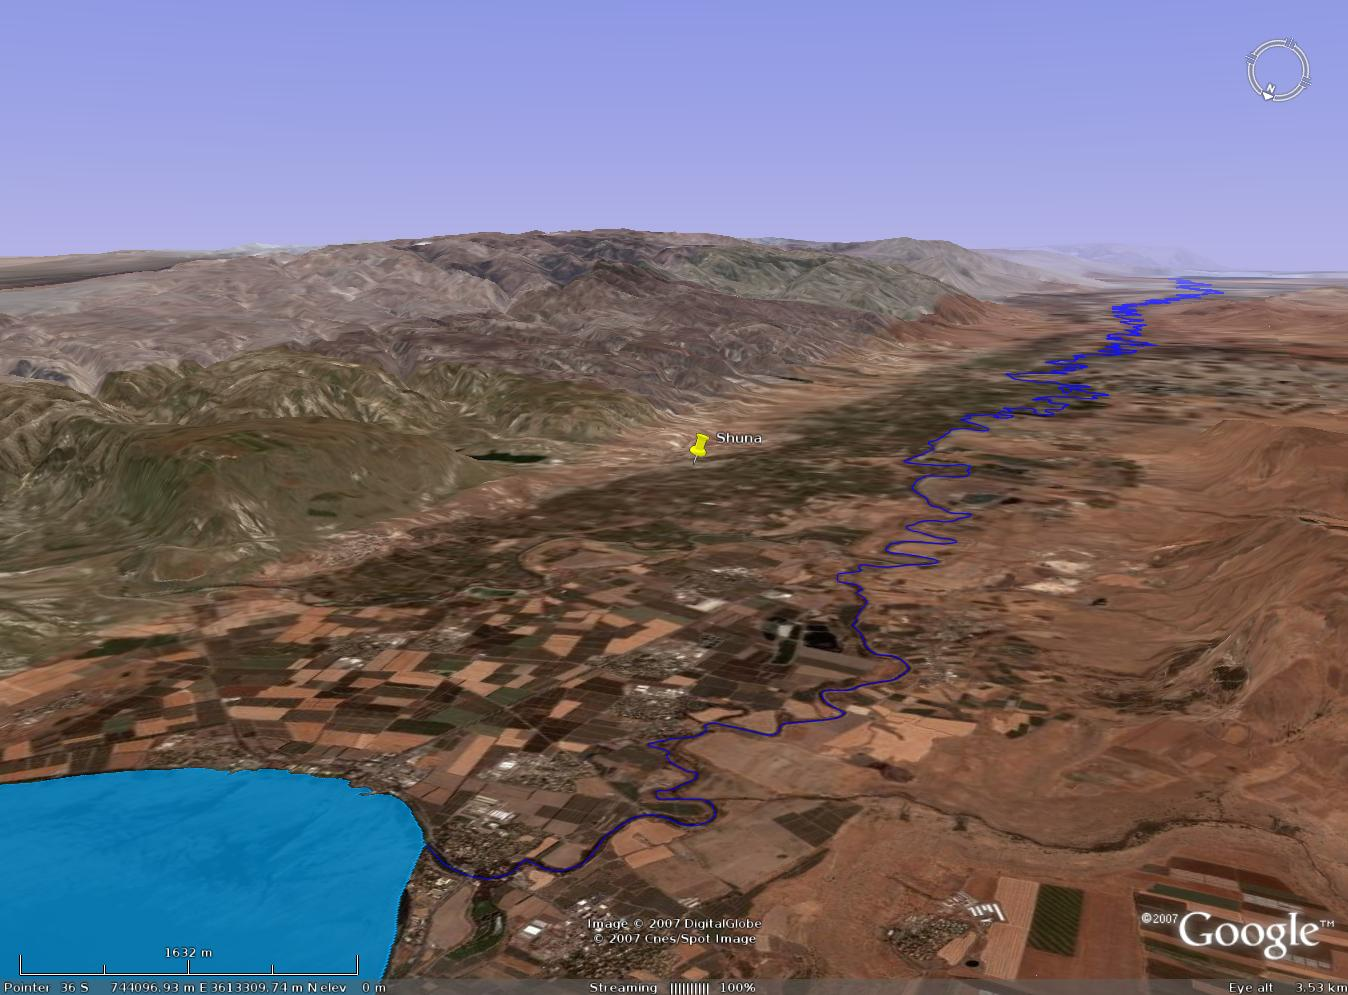
\includegraphics[scale=0.17]{./images/ShunaGoogleEarth3D.jpg}
  % img42.jpg: 800x600 pixel, 72dpi, 28.22x21.17 cm, bb=0 0 800 600
  \caption{\label{fig:shunaGoogleEarth}\textit{Looking South-South-East from Lake
    Tiberias Down the Jordan Valley towards Shuna.}} 
\end{figure}
\section{Background} 
  For an archaeologist, understanding the relationship that existed between
  people in the past and their landscape is very important.  People throughout
  time have relied on various plants and animals, wild or domestic, to provide
  them with the food they require to survive.  Regardless of the period in time
  being examined, a relationship exists between people and the space which they
  occupy.  A better understanding of this relationship can help to more
  confidently theorise about a range of issues in the reconstruction of past
  societies.  By piecing together clues gained through a combination of
  archaeological surveys, ethnoarchaeology, written records, oral traditions,
  and excavations, insights can be gained which can offer a more concrete
  understanding of the relationship people had with their landscapes, allowing
  archaeologists to better understand topics such as as short and long term
  impacts on the landscape, or social and economic organisation. 

  An understanding of long term impacts of ancient humans on their landscape
  can be useful for modern day researchers by providing insight into the potential 
  environmental impact of current human activities. In modern societies, urban 
  centres rely upon the surplus production of agricultural commodities provided 
  by farmers in the countryside.  This reliance necessitates a certain level of 
  organisation between rural and urban people.  By applying this same logic in 
  historical contexts, we can infer landuse patterns.

  Through careful study, a better understanding of the land use habits and
  patterns of these populations can unlock many interesting facets of culture
  and lifestyle.  By examining seeds, bones, and other items found at archaeological
  sites, archaeologists are able to determine dietary habits. From the relative
  quantities found estimates can be made of the importance each food source
  would have had in the diet.  The scale of production, for example, can help
  indicate whether crops were being cultivated for subsistence use or for more
  commercial purposes.  If there is evidence of surplus production of any particular crop
  or animal, this can be a possible indication that it was being grown
  commercially.  Other possible inferences include taxation, storage, redistribution,
  intensified farming, and craft specialisation, all of which can indicate 
  increased economic complexity.
\section{Process for computing landuse requirements} 
\label{sec:EarlyAttempts} 
  To learn more about how people interacted with their land, it is
  helpful to determine the area of land needed to support settlement
  populations and its likely distribution.  To locate the land being used, it is
  necessary to first know how \textit{much} land would have been needed to
  produce enough food to sustain the settlement.  Once this target for the area of land
  has been determined, the land surrounding the site must be classified as
  either suitable or unsuitable for each crop sown and each type of animal being
  raised.  The final, resultant map which LA produces, is a compilation of individual
  maps from each crop and animal, for which sufficient suitable land has been
  identified to meet the settlement's production requirements.
\section{Moving to a GUI} \label{GUI} 
  In late 2006, a BASH script was created running in a GRASS shell. This script
  found a specific area of classified, suitable land surrounding a point by
  starting at a point and moving outwards in a circle five meters at a time,
  checking each time to see if there was enough suitable land contained within
  the perimeter. As soon as it was equal to or greater than the target area, the
  loop was ended, and the solution was deemed found.

  The complexity of the animal and crop modelling made using BASH scripts very
  awkward.  While the BASH scripting approach worked well for a proof of
  concept, the implementation included a large number of hard coded variables and the
  solution did not provide a flexible environment for experimentation. For
  example, adding, removing or even editing different types of crops and animals
  to the analysis required heavy modifications to the BASH script.  The BASH
  script approach also had poor reporting capabilities and offered
  little 'hand holding' to the user as the analysis was carried out.

  Consequently we embarked on the development of a Graphical User Interface (GUI)
  based application (Figure \ref{fig:la544}), written in C++ and Qt4. This
  programming environment decision was largely motivated by a desire to
  capitalise on existing code bases from openModeller\footnote{openModeller is
  available at \url{http://openmodeller.sourceforge.net/}} and Quantum GIS
  (QGIS)\footnote{QGIS is available at \url{http://qgis.org}}.  For invoking
  GRASS tools we opted to use QProcess to launch GRASS commands in their own
  process and then implemented application logic to parse the results of each
  command from stdout.
\begin{figure}[htbp] %Proof of Concept
  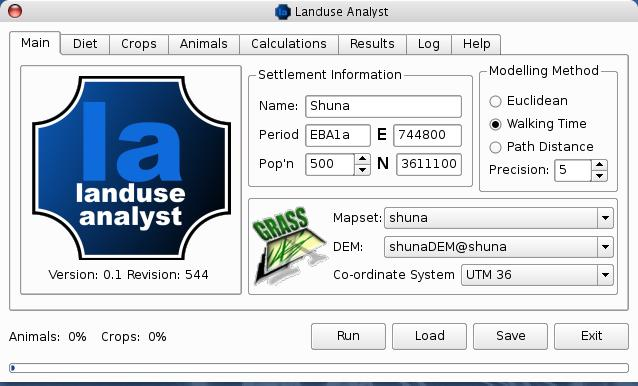
\includegraphics[scale=0.36]{./images/LanduseAnalyst544.jpg}
   % img42.jpg: 800x600 pixel, 72dpi, 28.22x21.17 cm, bb=0 0 800 600
  \caption{\label{fig:la544}\textit{LA's primary interface}}
\end{figure}
\section{Analytical functionality} \label{sec:Analytical Functionality}
  LA includes various routines for calculating the amount of land 
  the settlement needs.  Briefly, these can be outlined as follows:
  \begin{enumerate} 
    \item Breaking down the basic diet of the community into specific crops and
      animals being used for nourishment.  Each individual crop and animal needs to
      be expressed as a percentage of the peoples' diet.  This is estimated using
      proportions based on archaeological evidence such as faunal and
      paleobotanical remains discovered during excavations.  
    \item Calculating calorie targets for the crops and animals identified above.
    \item Calculating production targets which fulfil the calorie targets.
      Production targets are calculated in kilograms, and take into account factors
      such as calories per kilogram of produce, and what percentage of an animals
      weight is usable as food.  
    \item Calculating land area targets needed to satisfy the production targets.
      Each crop and animal is allocated a specific area target.  
    \item Carrying out a spatial analysis of the land surrounding the settlement
      to find land suitable for each crop and animal that satisfies the area
      targets.
  \end{enumerate}
\subsection{Determining calorie targets}
  Calorie targets are the first level of calculations done by LA and are
  determined through a number of steps (Figure \ref{fig:dietDiagram}), which
  are as follows.
    \begin{enumerate}
      \item \textbf{\textit{Basic Information}} - The user supplies LA with the
        population of the settlement, as well as the average daily calorific
        requirements of an average member of the population.  By multiplying
        these figures, the total number of calories required for the
        settlement is calculated (Figure \ref{fig:LADiet}).
      \item \textbf{\textit{Primary Dietary Components}} - This step works on
        the principle that calories can come from only two fundamental sources:
        plants and animals.
      \item \textbf{\textit{Detailed Dietary Components}} - At this step, the
        process gets split into two sections.  One section is for the Plant
        portion of the diet, and the other is for the Meat portion.
      \item \textbf{\textit{Crop/Animal Contributions}} - This value tells LA
        that this individual animal or crop comprises the indicated percentage of
        the calories being supplied by tame sources, which is the value from the
        previous step. Remember that this is a portion of the \textit{tame crop}
        part of the diet! 
        (See Fig. \ref{fig:dietMeatDiagram} and Fig.\ref{fig:dietCropDiagram}).
    \end{enumerate}
\begin{figure}[htbp] %dietDiagram
  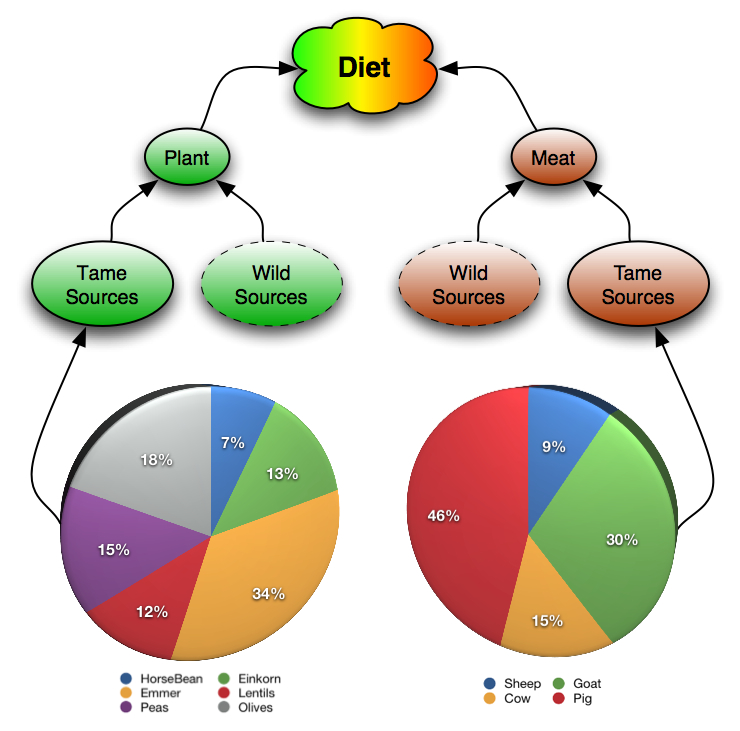
\includegraphics[scale=.31]{./images/dietDiagram.jpg}
  % dietDiagram.jpg: 740x731 pixel, 72dpi, 26.10x25.78 cm, bb=0 0 740 731
  \caption{\label{fig:dietDiagram}\textit{Conceptual diagram of a settlement's
    diet composition.}}
\end{figure}
\begin{figure}[htbp] %dietMeatDiagram
  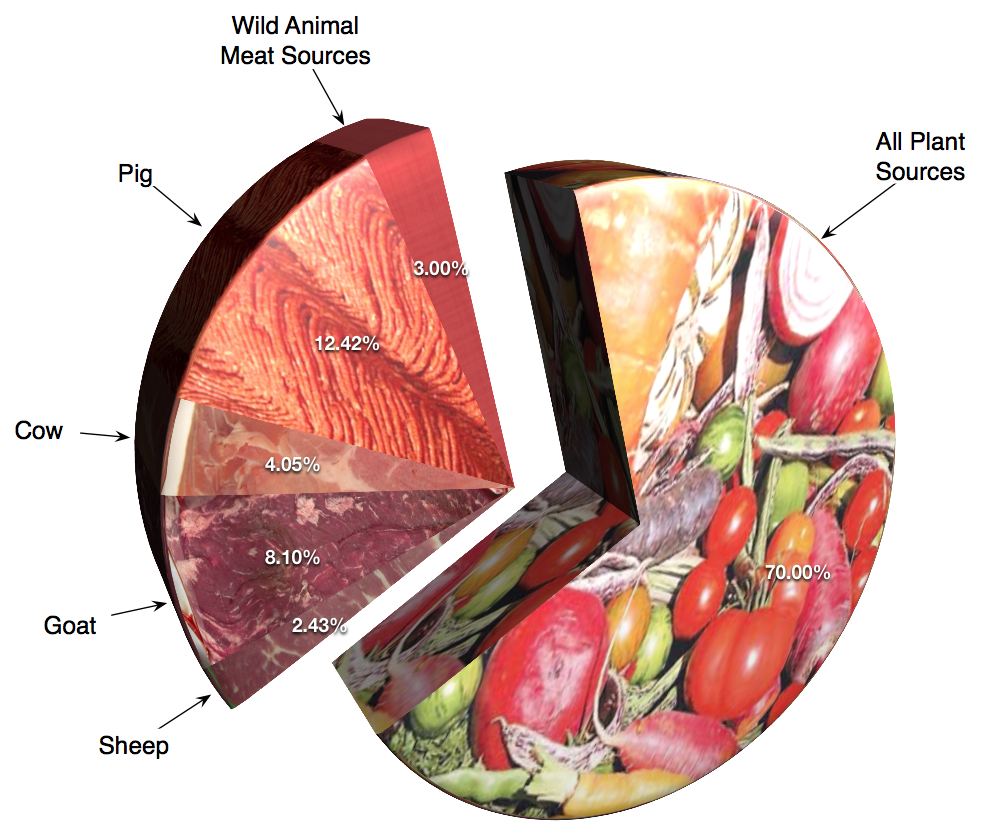
\includegraphics[scale=.23]{./images/fancyDietMeat.jpg}
  % dietDiagram.jpg: 740x731 pixel, 72dpi, 26.10x25.78 cm, bb=0 0 740 731
  \caption[Plant Portion of Diet]{\label{fig:dietMeatDiagram}\textit{Conceptual
    diagram of meat component of diet.}}
\end{figure}
\begin{figure}[htbp] %dietCropDiagram
  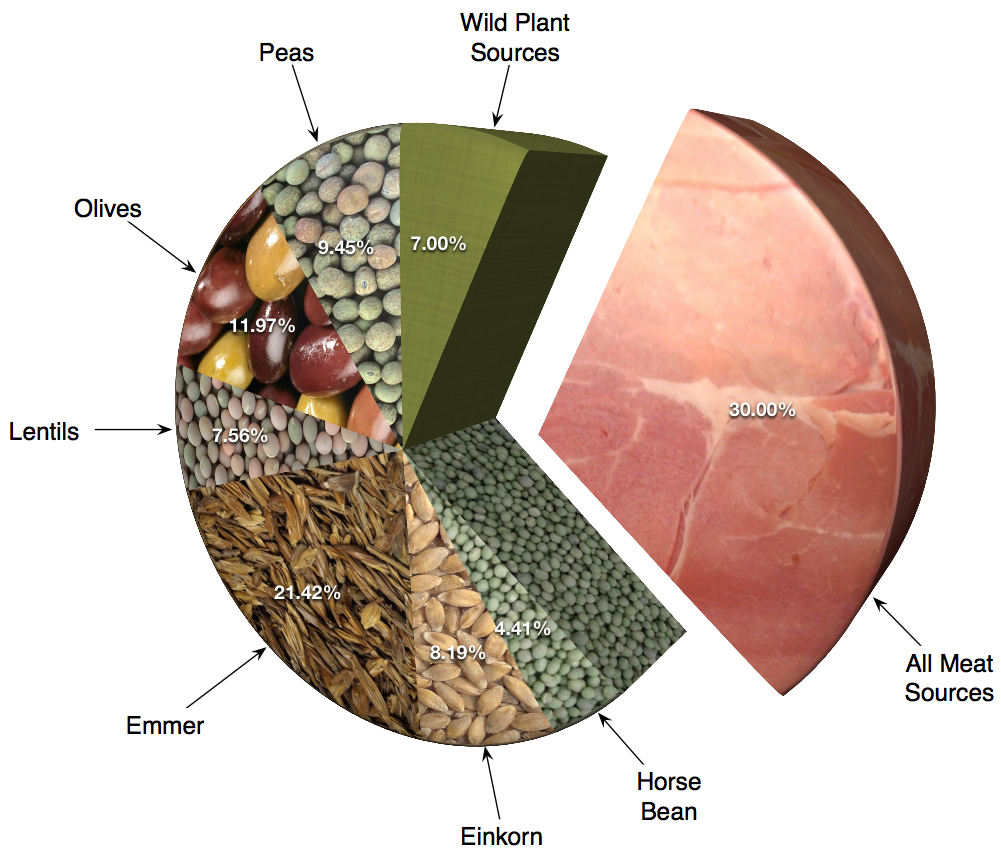
\includegraphics[scale=.2]{./images/dietFancyCrops.jpg}
  \caption[Plant Portion of Diet]{\label{fig:dietCropDiagram}\textit{Conceptual
    diagram of the plant component of diet.  Note that the input figures for
    percent of diet were: \textbf{HorseBean} $7\%$, \textbf{Einkorn} $13\%$,
    \textbf{Emmer} $34\%$, \textbf{Lentils} $12\%$, \textbf{Peas} $15\%$,
    \textbf{Olives}\ $18\%$.  These numbers translate to those shown above after
    processing as in Figure \ref{fig:dietDiagram}.}}
\end{figure}
\begin{figure}[htbp] %LADiet
  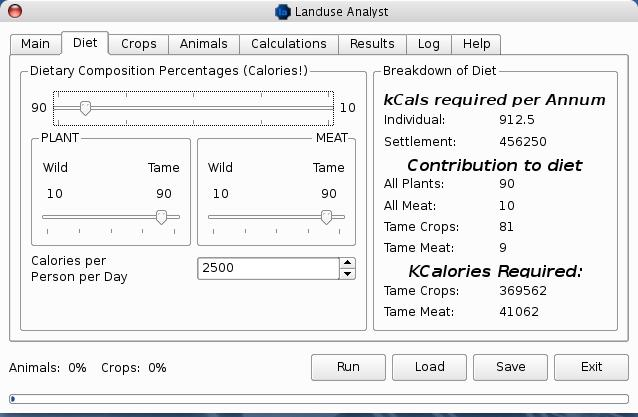
\includegraphics[scale=.355]{./images/LanduseAnalystDiet545.jpg}
  % LanduseAnalystDiet545.jpg: 638x417 pixel, 762dpi, 2.13x1.39 cm, bb=0 0 60 39
  \caption{\label{fig:LADiet}\textit{Diet Tab, LA}}
\end{figure}
  \subsection{Determining Production Targets}
    Production targets are measures of weight, and represent how many Kg of each
    crop and animal must be produced to satisfy the calorie targets calculated
    above.
  \begin{itemize}
    \item \textbf{Crops} - The user must supply the food value for each crop. 
      This is expressed as calories per kg.  Using the calorie targets and the
      user supplied food value, the model calculates a production target for each
      crop that is necessary to meet these needs.
    \item \textbf{Animals} - When animals get slaughtered, and only part of
      their carcasses are usable as food.  This usable part of their live weight
      is supplied by the users when they define the animal in the Animal Manager
      form, expressed as the percentage of their live weight which is usable as food.
  \end{itemize}
  \subsection{Determining Area Targets}
  Once production targets are calculated, it is possible to calculate area
  targets for each crop and animal by looking at yield values for plants, and
  grazing requirements for animals.  As with Production Targets, Area Targets
  are quite simple to compute for crops, but get very complicated for animals.
\section{Defining Characteristics}
 \subsection{Crops}
    A list of all crops that have been defined is found when the Crops tab is
    clicked (Figure \ref{fig:crop}).  Note that the user has the choice of
    selecting it for inclusion in the model, as well as being able to select
    different parameters from a drop-down list.  To the right of the drop down
    list is the crop's contribution to the tame plant portion of the diet using
    the currently selected parameter.  The total of these percentages must be
    equal to $100\%$ before the model will run, and the current total is always
    visible in the bottom left hand corner of the form.
\begin{figure}[htbp]
    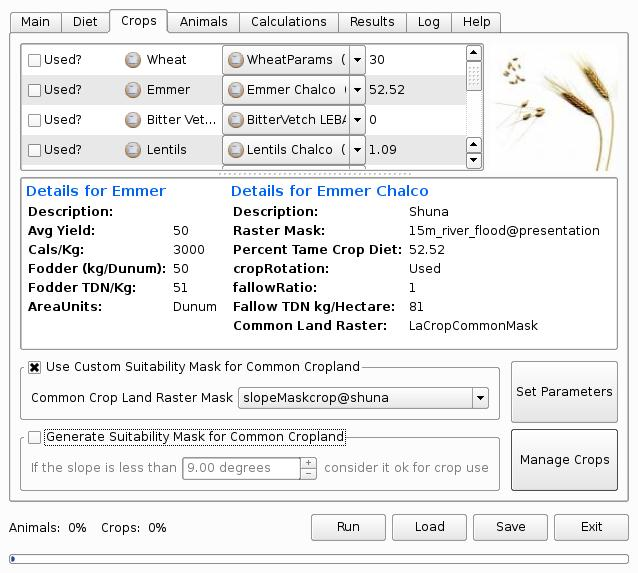
\includegraphics[scale=.36]{./images/LanduseAnalystCrops546.jpg}
    \caption{\label{fig:crop}\textit{Crops Tab, LA Version 0.1 Revision 544}}
\end{figure}

  \subsection{Defining Crops}\index{Crops!Defining}Every crop has unique
  characteristics, and LA splits these defining qualities into two
  main areas:  details of the plant and parameter settings.
    \subsubsection{Defining the Plants}LA uses seven input fields to define a
      plant (Fig.\ref{fig:cropManager}).

    \subsubsection{Crop Parameters}
    \label{cropParameters}
      Once you have defined the plants that are being grown as crops, Landuse
      Analyst needs to know the specifics of how each crop is being grown, as
      well as what portion of the settlement's diet it provides (Fig.
      \ref{fig:cropParameters}).  It must also know what land is capable of
      growing each crop by selecting either Common or Specific Land Suitability masks
      (keeping in mind that if Specific Land is selected, the Raster Mask must
      be selected from the drop down list).  The two major entries, however,
      involve \textit{crop rotation} and the selection of \textit{suitability masks}.
    \subsubsection{Crop Rotation}
    \label{cropRotation}
      A common farming technique still used widely even today is the practise of
      resting your cropland every growing season or so.  This is called
      \textit{crop rotation} (Figure \ref{fig:cropParameters}) and is critical
      to the process of determining how much land is required for food production,
      as it can more than double the area target for a crop.  Complicated crop 
      rotations are possible in LA, and the process of setting this up are
      explained in detail in the Help section of the program itself.

\begin{figure}[htbp]
  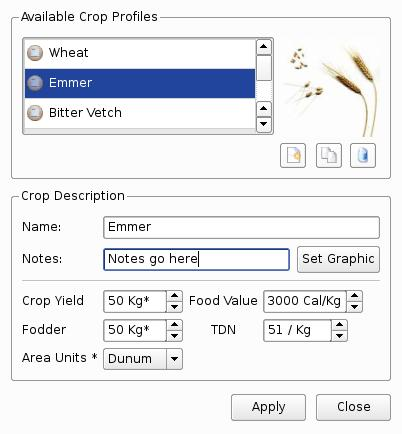
\includegraphics[scale=.59]{./images/cropManager.jpg}
  % cropManager.jpg: 402x434 pixel, 762dpi, 1.34x1.45 cm, bb=0 0 38 41
  \caption{\label{fig:cropManager}\textit{Crop Manager, LA}}
\end{figure}
    Another important aspect of defining crop rotation concerns animals.  It is
    possible for animals to graze the fallow land, which will reduce the amount
    of grazing land otherwise required to sustain the animals.  In order to
    know how much contribution the fallow land makes, it is necessary to know
    the food value of the fallow land.  Using the ratio of crop land to fallow
    land along with the food value of the fallow land allows LA to
    accurately adjust the grazing land requirements for the animal herds.  How
    this is done is explained in detail in the following section.

\begin{figure}[htbp] %crop parameters
  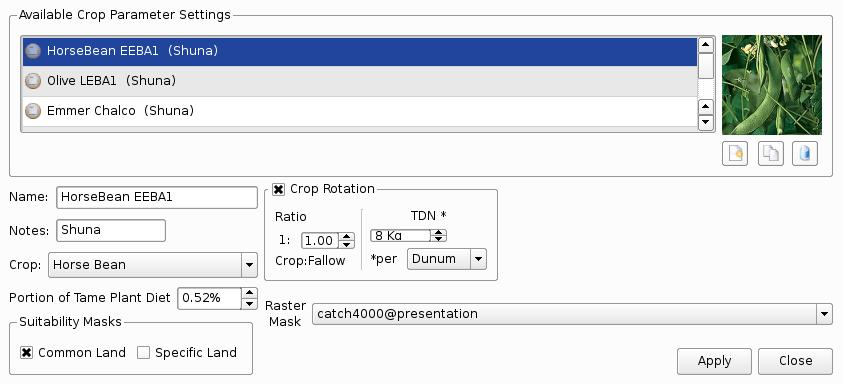
\includegraphics[scale=.27]{./images/cropParameters.jpg}
  % cropParameters.jpg: 842x384 pixel, 762dpi, 2.81x1.28 cm, bb=0 0 80 36
  \caption[Crop Parameters]{\label{fig:cropParameters}\textit{Crop
    Parameters form for setting the particulars of the crop.}}
\end{figure}
  \subsection{Animals}
    Animals are difficult to calculate area targets for because their land
    requirements are largely based on their numbers, and a herd of adult
    females large enough to sustain a steady supply of offspring with numbers
    enough to keep the production targets met has to be added into the equation
    as well.  In addition, animals can graze fallow crop land, eat fodder from
    the crops being grown, and graze other types of land.  LA takes these
    interactions into account in its computations.
    Herd Size determination is perhaps the single most difficult calculation
    that LA performs.  Added to the complexity of this is the problem that different
    animals have different dietary requirements, and even further, even if they
    are the same, they require different amounts of feed depending on things
    like whether they are pregnant or lactating.  To further complicate the issue,
    not all land that can be grazed has the same food value to the animals.

    LA does, however, address these issues.  One of the first things a user must
    do when using Landuse Analust is to define all of the crops and animals that
    the settlement used.  During this process the users provides information
    about aspects including (for animals) information
    relating to their dietary requirements, their reproduction cycle, and their
    grazing preferences.
    \subsubsection{Defining Animals}
    \label{definingAnimals}
      Animals present several challenges that plants do not.  For starters, a
      certain number of females must be kept solely as breeding stock, and this
      number must be calculated based upon production requirements.  Secondly,
      the possibility exists that part of the animals' diet was from either
      straw/chaff left over from harvesting crops, or directly from harvested
      grain.  In the case of grain being used as feed, the amount used must be
      considered when determining the production targets for the crops. 
      Thirdly,if crop rotation was happening and fallow land was present, there
      is the possibility that this was used as grazing land, and would therefore
      reduce the amount of natural grazing land required.  This also adds
      complexity to the crop models because grazing fallow land adds fertiliser,
      potentially increasing yields.  This phenomenon can be factored in to
      Landuse Analyst by manually adjusting the expected yield of the affected
      crops.

      Version 0.1 of LA allows animals to use fodder as food.  The amount of the
      contribution of fodder is expressed as an overall percentage of their diet
      in terms of calories.  Furthermore, the model provides separate inputs for
      fodder (straw/chaff) as well as straight grain.  When setting up the
      model, the user supplies fodder production levels for the crops, as well as
      caloric levels for the fodder.
\begin{figure}[htbp]
  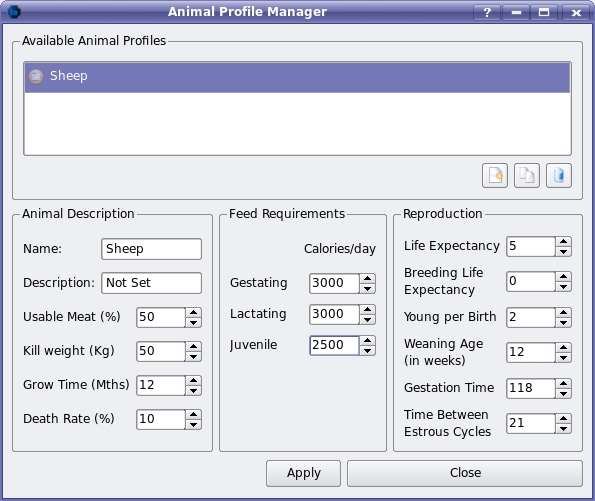
\includegraphics[scale=.38]{./images/animalManager.jpg}
  % cropManager.jpg: 402x434 pixel, 762dpi, 1.34x1.45 cm, bb=0 0 38 41
  \caption{\label{fig:animalManager}\textit{Animal Manager, LA}}
\end{figure}
    \subsubsection{Animal Characteristics}
      LA uses several input variables  to define an animal (Fig.
      \ref{fig:animalManager}).  Two items which are worth further discussion
      are the Common and Specific Land options.
      \begin{itemize}
        \item \textit{\textbf{Common Land}} - Sometimes land is suitable for
          grazing by more than one type of animal. LA allows you to
          designate one suitability mask as common grazing land. Note that you
          can specify an animal to use both common land and specific land at the
          same time. If this is the case, equal preference is given to all
          animals grazing the common land. This is not always ideal, as it may
          have been the case that some animals were given preference to the
          common land if the other suitable land was further away than the other
          animals using it.  (A workaround for this problem is that LA
          produces classified maps of the land being used, so if it is
          the case that you find one animal being forced to travel much further
          than others, you can simply change the settings to balance this. This
          can be accomplished by removing the other animals one at a time from
          using the common grazing land. It may be the case, however, that there is no
          ideal solution, and that they simply had to travel the extra
          distance.)
        \item \textit{\textbf{Specific Land}} - Sometimes you may want to
          specify that land is suitable for grazing by only one type of animal.
          LA allows you to designate a land suitability mask as
          being unique to that animal.  Note that you can specify an animal to
          use both common land and specific land at the same time. For more
          detailed information on this, see the help section of LA.
      \end{itemize}
\begin{figure}[htbp]
  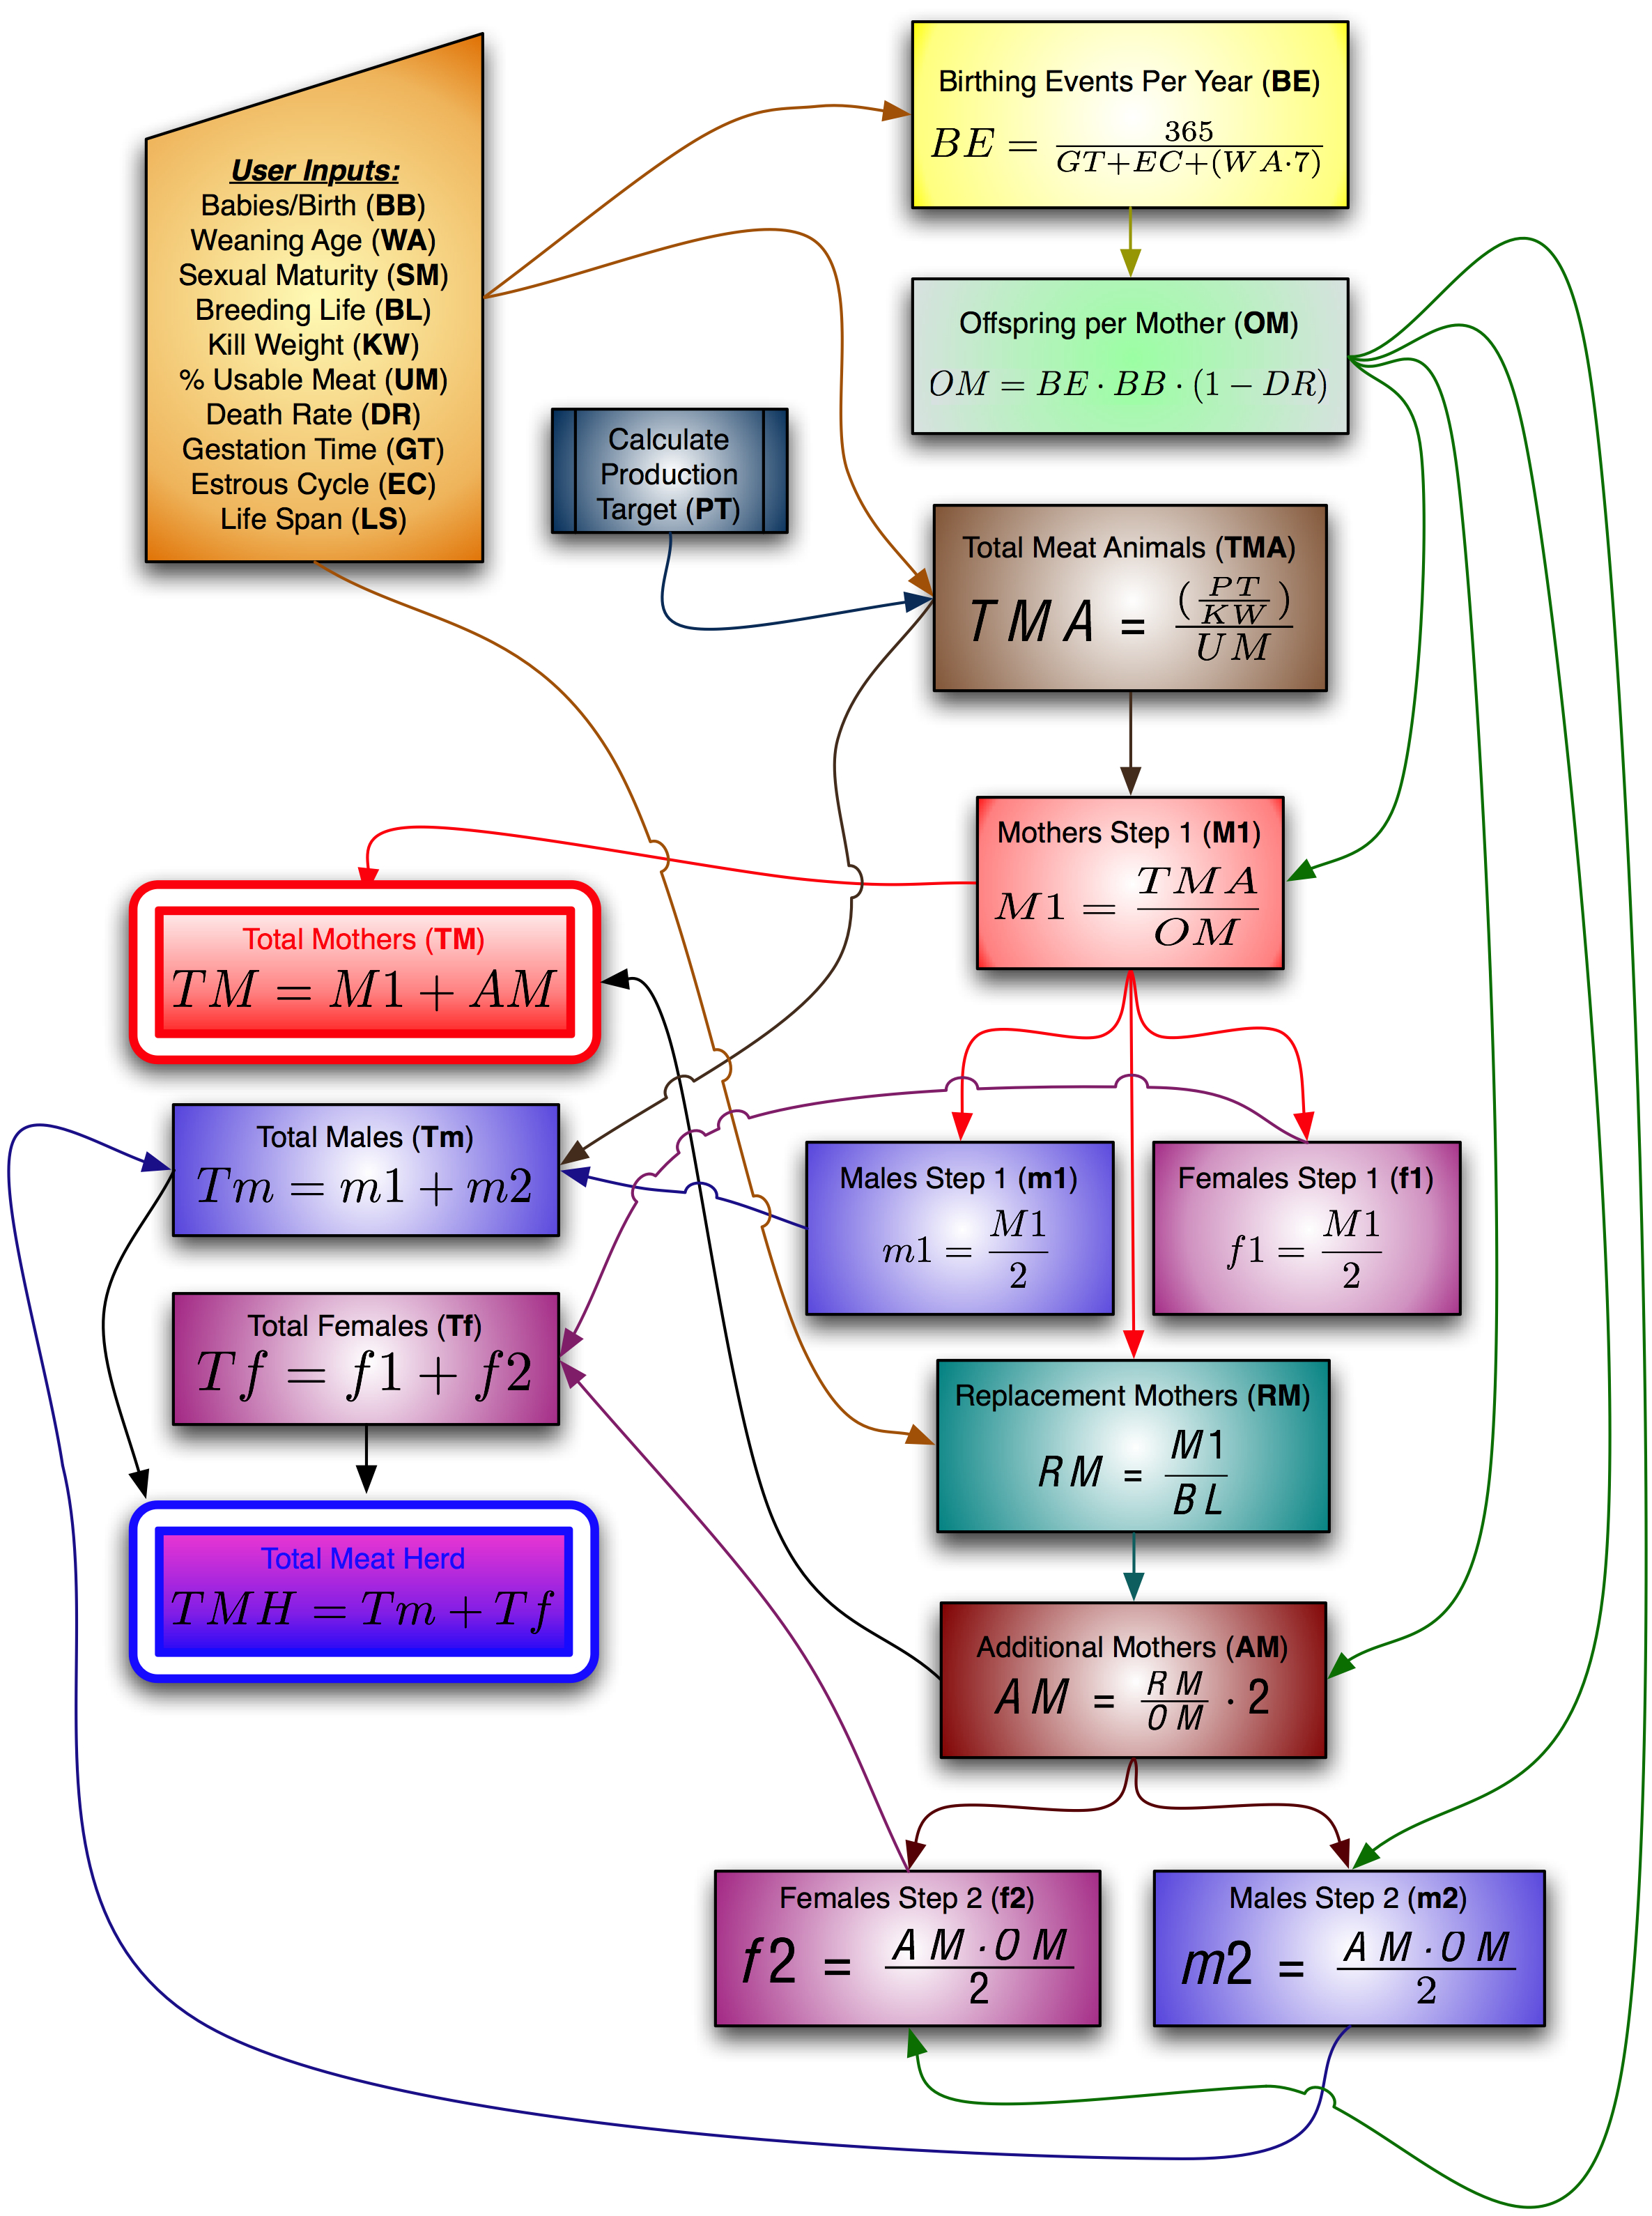
\includegraphics[scale=.4]{./images/animalHerdSize.jpg}
  % animalHerdSize.jpg: 2371x3180 pixel, 300dpi, 20.07x26.92 cm, bb=0 0 569 763
  \caption[Animal Herd Size Calculation]{\label{fig:herdSize}\textit{Animal
    Herd Size Calculation - This diagram assumes that the production target has
    already been worked out.  Units for input variables are: \textbf{WA}-days,
    \textbf{SM}-months, \textbf{BL}-years, \textbf{KW}-kg,
    \textbf{DR}-percentage, \textbf{GT}-days, \textbf{EC}-days,
    \textbf{LS}-years, \textbf{PT}-kg.}}
\end{figure}
  \subsection{Herd Size Calculation}
    The size of the herd required to sustain a particular amount of meat for a
    population is crucial for determining an area target for each type of animal
    raised.  An algorithm generic enough to make this calculation for any animal
    that has been defined in LA was created. By taking the Production
    Target and several user inputs, the total number of adult females (Mothers)
    and animals being raised for meat (Meat Animals) can be approximated. This
    process is outlined in Fig. \ref{fig:herdSize}.
\section{Land Redesignation}
  Another notable feature of LA is land redesignation.  Land that is suitable
  for the production of crops is almost certainly suitable for grazing as well. 
  For this reason, LA performs all of the cropland functions first.  Once the
  area targets for all crops have been satisfied, all of the unallocated land
  previously classified for use by crops is redesignated as being suitable for
  common grazing land. 
\section{Catchment creation methods} 
  When searching for land that meets the area targets, LA starts at
  the coordinates of the settlement and moves outward to a point where the land
  contained within equals the area target.  LA implements three
  different methods for searching outwards from the settlement.  The key
  difference between the three methods is the way in which a cost-surface is
  generated, which we will now examine.  All three methods currently used by LA
  require a \textbf{D}igital \textbf{E}levation \textbf{M}odel (DEM) to generate
  the cost surfaces.
    \subsubsection{Euclidean} \label{subsubsection:Euclidean} 
      This method ignores all topographic features of the landscape when moving
      outwards from the site.  Essentially we are drawing circles around the site,
      with the site right in the middle.  Drawbacks to using this method exist.
      Whilst moving across a landscape, people are affected by slope, rivers,
      landcover, etc.  Circles are just convenient when there is no easy way to
      calculate with an alternative method.  The primary reason for its inclusion
      as a catchment area creation method in LA is to provide the user
      with the option of seeing the difference between this rather simplistic
      approach and the other two methods.
    \subsubsection{Path Distance}
      Path Distance is a cost surface creation method that looks at elevation data
      from a DEM and calculates distance from the site taking into account the
      extra distances travelled going up or down slopes.
    \subsubsection{Walking Time}\index{Walking Time}
      Walking Time is likely going to be the primary choice of the three methods of
      creating catchment areas in LA.  The cost surface that is
      generated for this method (Figure \ref{fig:rwalk}) uses a DEM to calculate
      how long it would take to walk from a starting point (the site, or ZERO on
      the cost surface) to all points on the DEM within a five hour walk ($18,000$
      seconds). Five hours is simply the time used for this case
      study\footnote{This number is currently hard coded. Future versions will
      allow the user to edit this value.} This creates a cost surface with values
      from $0$ to $18,000$ (Figure \ref{fig:rwalk}).  
\begin{figure}[htbp] 
  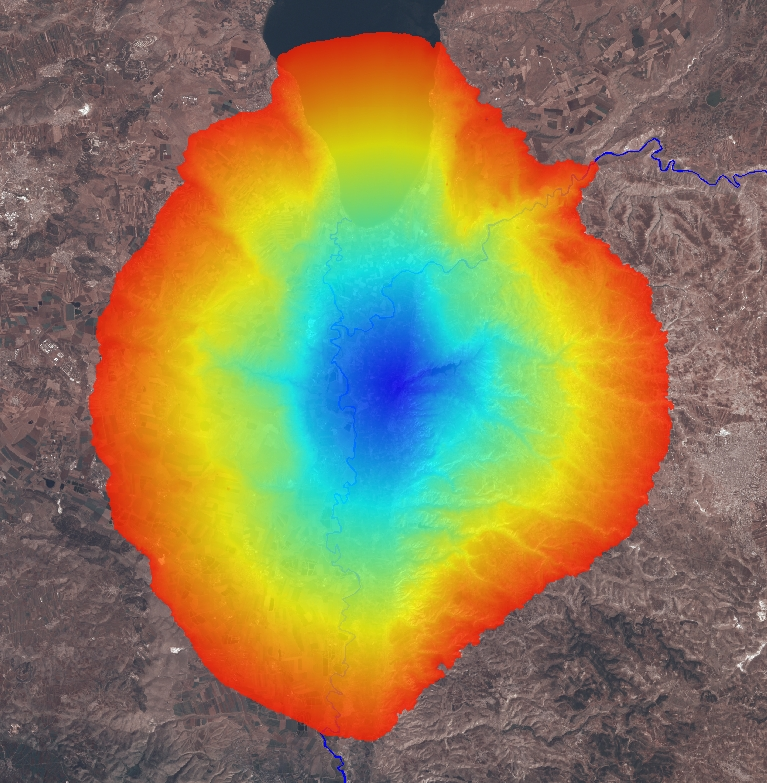
\includegraphics[scale=0.29]{./images/rwalkShuna.jpg}
  %caption of the figure
  \caption{\label{fig:rwalk}\textit{LA generated this using the GRASS module r.walk.}}
\end{figure}
\section{Land suitability raster masks} 
  The land suitability masks must be binary rasters, meaning that the cells of
  the raster file only contain 0 or 1 (NULL values are currently not supported).
  The land that is deemed suitable for use should be set to a value of 1, and the
  rest of the land is set to 0.  This binary raster  can then be multiplied by a
  selection layer (as created by either Walking Distance, Path Distance,
  or Euclidean methods).  This selection layer (also a binary raster) grows in
  size until enough area is
  found within it's bounds - identifying the land to be analysed.

  In the current version, the software gives the option using three different
  methods for landuse classification.  They are: 
  \begin{enumerate} 
    \item  Use only the user supplied classification map (a binary mask) 
    \item  Use minimum and maximum slope values to create a classification map
      which will be used exclusively.  This can be done for common crop land and
      common grazing land independently.  For example, the user might stipulate
      $0^\circ \leq m \leq 9^\circ$ for crops and $9^\circ < m \leq 15^\circ$
      for grazing land, where $m=slope$.  
    \item  Using a combination of the two classification maps.  Slope can be
      chosen to either add to or subtract from the user supplied map, or 
      alternatively, the user supplied map can either add to or subtract from
      the slope map.  This combination of the two can be very useful if, for 
      example, a user wishes to use a soil classification map as the primary
      indication of landuse suitability, but refine that map by taking out the
      land they consider too steep for use. In this case the program generated
      slope masks would be subtracted from the user supplied (soil) classification map.  
  \end{enumerate}
\begin{figure}[htbp] %Location
  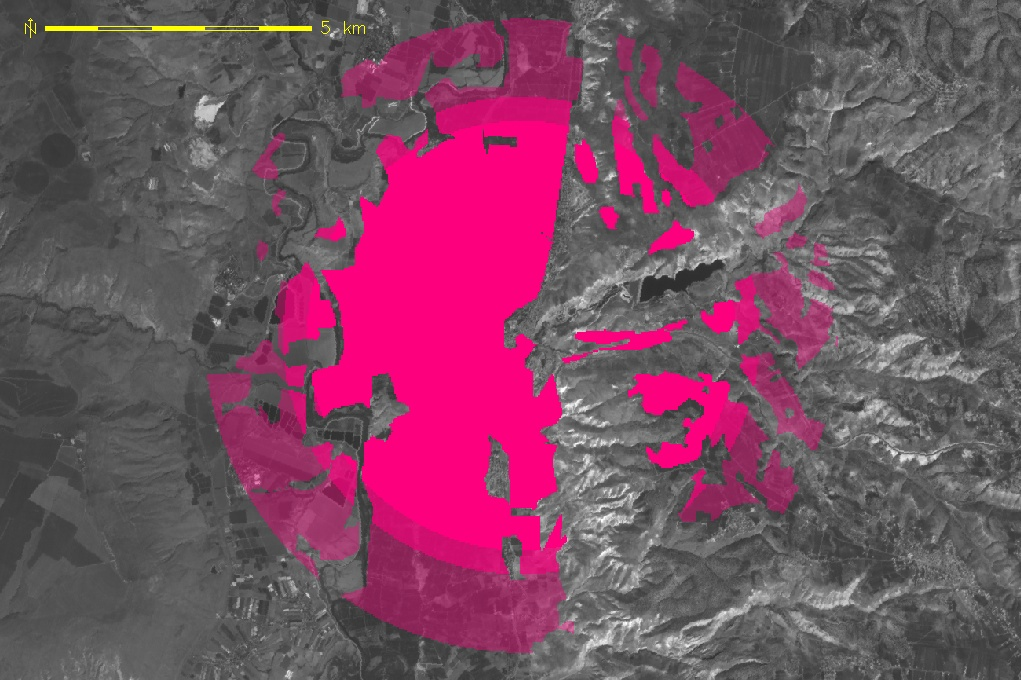
\includegraphics[scale=0.225]{./images/landcatchment.jpg}
  % img42.jpg: 800x600 pixel, 72dpi, 28.22x21.17 cm, bb=0 0 800 600
  \caption{\label{fig:landCatchment}\textit{Results which identified the suitable land
    surrounding Shuna using Euclidean method. The different shades represent
    different settlement populations.}}
\end{figure}
\section{Finding the land} 
  From a GIS point of view, one of the greatest challenges of this project was
  developing a method for finding the outer extent (or boundary), within which
  the combined area of suitable land satisfies the target area.  The usable land
  surrounding a settlement is almost certainly not going to be contiguous, but
  rather comprised of multiple, irregularly shaped polygons. A further
  complication is the fact that some of the irregularly shaped polygons may
  be bisected one or more times by the 'boundary line'.

  In order to find the suitable land required to produce enough food to sustain
  the settlement that is in closest proximity, a conditional loop is used which
  defines the outer extent of the catchment area, and then calculates the area of
  suitable land contained within it.  This process is identical for all analysis
  methods.  The earliest versions of LA started at the closest point to the site
  that could potentially solve the problem \footnote{The closest point, or
  minimum radius, is a perfect circle equal in area to the target.}, and then
  moved steadily outwards until the area target was found.  The amount to move
  outward in each step was provided by the user, and might have been a
  value like 30 (which in the case of walking distance meant 30 seconds, on  a
  cost surface of 20,000.  This would mean that potentially, there would have to
  be $\frac{20,000}{30}$ or nearly 7000 iterations!)
  The basic steps involved were:
  \begin{enumerate} 
    \item Set the initial boundary at which to start the analysis
    \item Calculate the area of suitable land found within this boundary 
    \item If the area of land required has been satisfied, write the results to
      a new file for that item and exit the loop 
    \item Increase the value of the analysis boundary 
    \item Repeat the loop (starting at Step 2)
  \end{enumerate}
  This method proved extremely time consuming;  If even 3,500 loops, which is
  about half of the cost surface map, was required, and each loop took as little
  as 45 seconds, the computation time was nearly 44 hours.  Multiply this, then,
  by the number of individual crops and animals in the model and the run time 
  suddenly needs to be expressed in days or weeks.  To increase the efficiency,
  a modified binary search is now used.  This involved a somewhat different 
  approach.  Instead of using a step amount, a percentage is used.  This
  percentage value is called the \textit{Precision}.  

  The area of land deemed by LA as equalling the current area target gets
  changed into a target range $\pm$ the precision value multiplied by the 
  target area. If a value of $5\%$ is entered, and the area target is 100
  hectares, LA accepts $100 \pm(\frac{100 \cdot 5\%}{2})$ (which is $97.5$
  to $102.5$ hectares) as the target area.  

  The loop uses three terms, $CurrentMidValue$ $FirstValue$ and $LastValue$.
  At the beginning of the process, $FirstValue=0$ and $LastValue=18,000$
  which coincides with the full extent of the cost surface.  $CurrentMidValue$
  is calculated within the loop.  The loop works like this:
  \begin{enumerate} 
    \item Set the analysis boundary: $CurrentMidValue=\frac{FirstValue +
      LastValue}{2}$.  
    \item Calculate the area of suitable land found within the boundary whose
      outermost boundary is $CurrentMidValue$ 
    \item If the contained area falls within the target range, write the results
      to a new file and exit the loop 
    \item If the contained area is more than the maximum value in the target
      range, set a halfway between $FirstValue$ and $CurrentMidValue$. This is
      done by making $LastValue=CurrentMidValue$ and then returning back to step
      number one.  (Note $FirstValue$ remains unchanged.) 
    \item If the contained area is less than the minimum value in the target
      range, set a halfway between $LastValue$ and $CurrentMidValue$. This is
      done by making $FirstValue=CurrentMidValue$ and then returning back to step
      number one.  (Note $LastValue$ remains unchanged.) 
  \end{enumerate}
  By using this method, the \textit{maximum} number of steps in the loop is 17.
  This method of searching for the area targets made a huge difference in LA's
  speed.  A typical 'run' on a decent computer system is now $\approx$ 2 to 3
  minutes, compared days and weeks using the original method.  This allows a
  user to now examine many different variations of an entire model quickly and
  easily, even on an average computer system.

  Finally, at the end of the process, LA produces maps which clearly show
  which land people in the settlement were likely to have been engaged with, and
  for what purpose they were using it (Figure \ref{fig:caseStudy}).
\begin{figure}[htbp] %Location
  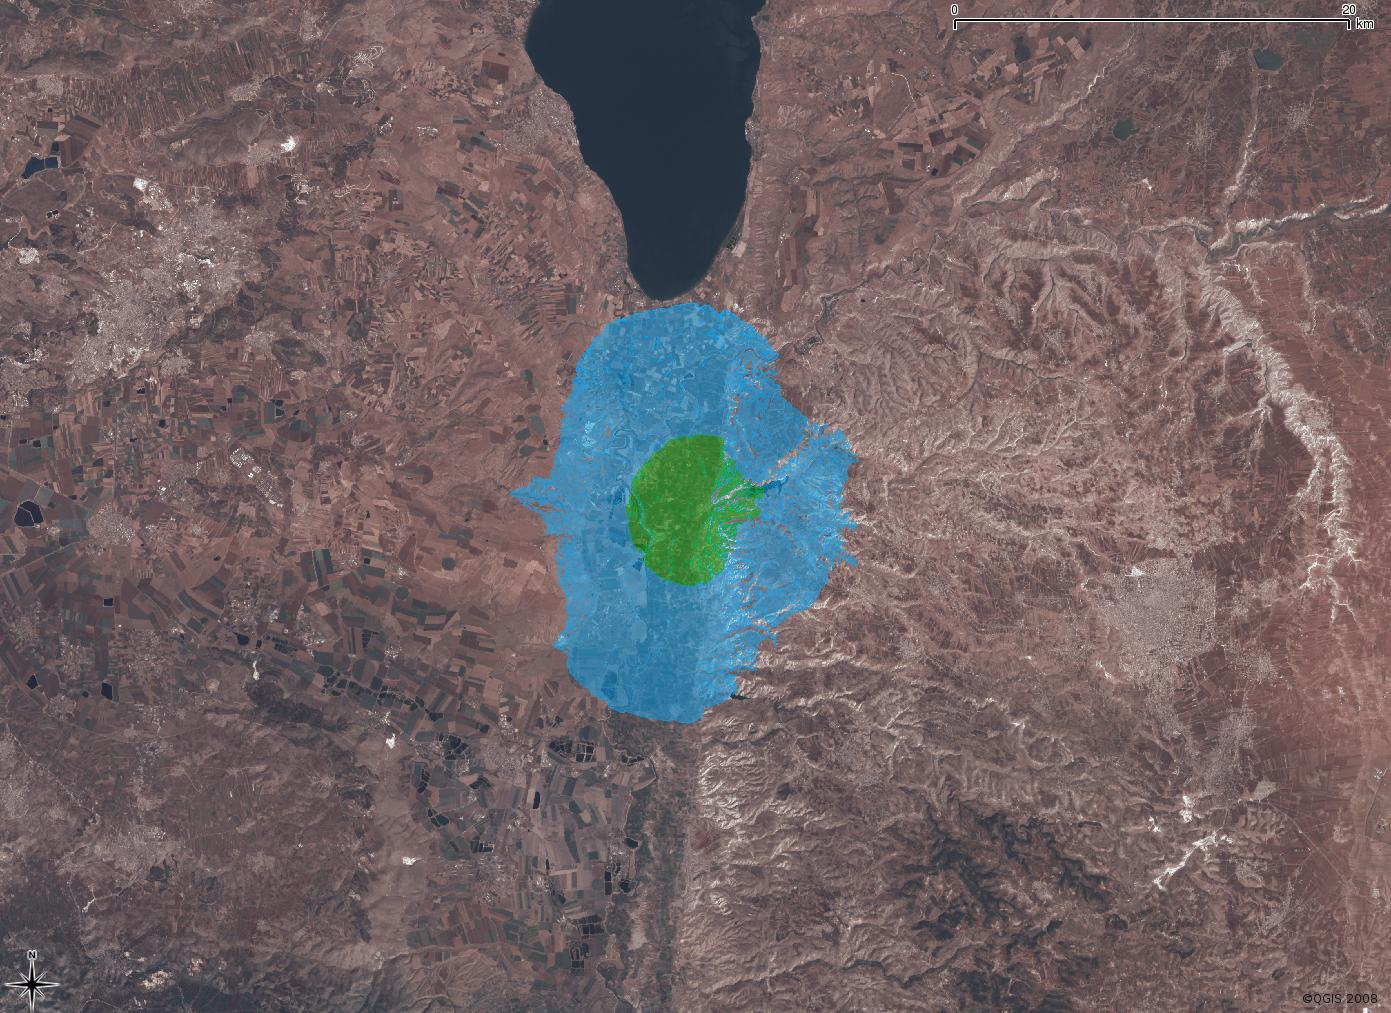
\includegraphics[scale=0.22]{./images/LEB130009010FallowSlope.jpg}
  \caption{\label{fig:caseStudy}\textit{Sample results for Shuna, Late Early Bronze Age,
    Population 3000, 90\% plant and 10\% meat.  Green is for cropland, blue grazing land.  Walking Time
    was used to create the cost surface, and slope was used for mask generation.}}
\end{figure}
\section{Future development} \label{FuturePlans} 
  LA is still in the early stages of its development and many
  improvements to usability and application capabilities are planned. That said,
  the application is already capable of producing useful results (though more
  testing is still needed) in a more flexible, user friendly and efficient
  manner than the original BASH prototype.

  There are many routes that LA can take from this point with
  respect to it's future development; it can continue on as a standalone
  application, or turn into a plugin for another application like openModeller
  or QGIS.  Before these decisions are made, however, the features in the current
  version must be finalised and implemented.  Some features which are currently
  in the planning phase are network analysis  for inter-site relationships,
  experiment settings, where the model can be set to run a given number of times
  using different input variables, and report generation complete with graphs
  and maps. 

  The network analysis feature will look at all contemporaneous sites in a given
  area, and examine production potential.  If a site can potentially produce
  excess meat, but falls short in cropland, it will look to neighboring sites to
  see if they can make up the difference.  If there is a potential for trade or
  supplementation, the most efficient walking routes can then be found using
  r.drain on a cost surface generated with r.walk.  This could potentially show
  the likely pathways between sites, as well as how intensively used they might
  have been.  Taking this further, one might look for places where these routes
  merge, or cross, which might be an indicator for a potential archaeological
  site which has yet to be discovered.

  The current version of LA requires that every scenario be modelled
  manually and separately.  For example, one might wish to look at how adjusting
  the yield of crops would affect the land requirements to simulate drought
  years.  One might also want to compare the results of different dietary
  proportions of meat content to plant content.  With the experiment module, it
  will be possible to have the software automatically cycle through all of these
  different scenarios automatically.

  Drawing much on the work done in openModeller, there is also the hope that it
  will be possible to have LA compile presentation quality reports,
  complete with spreadsheets and graphs.  This will be a great time saving
  feature.  In addition, this will provide a consistency that will make it much
  easier to systematically compare results with other users.

  Anyone interested in knowing more about this project, or better yet, in
  contributing to it, please don't hesitate in contacting us.


%etc.  \end{smallverbatim}


%if you want to cite please use:

% \cite{name:year} or \citep{name:year}

%.... revealed by \cite{herborg:2003} if it shall be in parentheses use
%\citep{herborg:2003}


%End of text.



\begin{footnotesize}
%\begin{thebibliography}{99}

%\bibitem[Herborg et~al. (2003) Herborg, Bentley, Clare, Rushton]{herborg:2003}
%L.M. Herborg, M.G. Bentley, A.S. Clare, S.P. Rushton (2003) \newblock The
%spread of the Chinese mitten crab (Eriocheir sinensis) in Europe; the
%predictive value of an historical data set.  \newblock {\em Hydrobiologia}
%503: 21-28.


%\end{thebibliography}
\end{footnotesize}


\address{Jason Jorgenson\\ University of Liverpool\\
\url{http://www.arkygeek.com} (under development)\\
\email{jjorgenson@gmail.com}}

\address{Tim Sutton\\ Centro de Referncia em Informao Ambiental, CRIA\\
\url{http://cria.org.br}\\
\email{timlinux@linfiniti.com}}

%%% Local Variables:
%%% mode: latex
%%% TeX-master: main_document.tex
%%% End:
